\chapter[Primjena algoritamskih paradigmi na probleme iz aritmetike]{Primjena algoritamskih paradigmi na probleme iz aritmetike}

U ovoj glavi razmatramo primjenu algoritamskih paradigmi predstavljenih u prethodnom poglavlju na odabrane probleme iz aritmetike i teorije brojeva. Cilj je pokazati kako se različiti pristupi dizajnu algoritama, poput grube sile, podijeli-pa-zavladaj, dinamičkog programiranja i drugih paradigmi, mogu koristiti za efikasno rješavanje matematičkih problema.\\

%ISHODI UCENJA:

Nakon uspješnog savladavanja sadržaja ove glave student će biti u stanju da:

\begin{itemize}
	\item primijeni prethodno obrađene algoritamske paradigme na rješavanje
	problema iz elementarne aritmetike i teorije brojeva;
	
	\item objasni i implementira Eratostenovo sito za efikasno određivanje
	prostih brojeva u zadanom intervalu;
	
	\item implementira postupke faktorizacije cijelih brojeva i analizira
	njihovu vremensku složenost;
	
	\item izračunava binomne koeficijente primjenom rekurzivnog pristupa
	i dinamičkog programiranja te uporedi njihove performanse;
	
	\item objasni i implementira Hornerov metod za efikasno izračunavanje
	vrijednosti polinoma;
	
	\item analizira vremensku i prostornu složenost algoritama za razmatrane
	aritmetičke probleme i uporedi različite pristupe njihovom rješavanju.
\end{itemize}

\section{Eratostenovo sito}

\begin{definition}
	Broj $n \in \mathbb{N}$ naziva se \textit{prostim brojem} ako je djeljiv isključivo sa $1$ i samim sobom.
\end{definition}

Na primjer, prvih pet prostih brojeva su: $2, 3, 5, 7, 11.$ Broj $6$ nije prost jer je, pored brojeva $1$ i $6$, djeljiv i sa $2$ i sa $3$.

\medskip

Posmatrajmo sljedeći problem:
\begin{quote}
	Odrediti sve proste brojeve manje ili jednake vrijednosti $N$.
\end{quote}

Jedan jednostavan pristup zasniva se na paradigmi grube sile. Za svaki broj iz intervala $[2,N]$ provjeravamo da li je prost koristeći sljedeću proceduru:

\begin{minted}{python}
	def prost(n):
	
	    for i in range(2, n // 2 + 1):
	        if n % i == 0:
	            return False
	
	    return True
	
\end{minted}

Ova procedura u najgorem slučaju izvršava $O(n)$ operacija za broj $n$. Kako se poziva za približno $N$ različitih brojeva, ukupna vremenska složenost ovakvog pristupa iznosi $
O(N^2).$

Za veće vrijednosti parametra $N$ ovakav pristup postaje neefikasan.

\medskip

Efikasnije rješenje daje algoritam poznat kao \textit{Eratostenovo sito}. Njegova osnovna ideja zasniva se na sljedećem zapažanju:

\begin{quote}
	Ako je broj $p$ prost, tada nijedan njegov višekratnik
	$ 2p,3p,4p,\ldots$	ne može biti prost.
\end{quote}

Zbog toga, nakon što identifikujemo prost broj $p$, svi njegovi višekratnici mogu se odmah eliminisati iz daljeg razmatranja.

Algoritam počinje skupom svih brojeva od $2$ do $N$. Najmanji broj koji još nije eliminisan proglašava se prostim, nakon čega se svi njegovi višekratnici označavaju kao složeni brojevi. Postupak se zatim ponavlja za naredni neoznačeni broj. Na taj način se progresivno filtriraju svi složeni brojevi, dok u ``situ'' ostaju upravo prosti brojevi.

Proces se završava kada više nije potrebno eliminisati nove višekratnike. Preostali neoznačeni brojevi predstavljaju sve proste brojeve manje ili jednake vrijednosti $N$.

\medskip

Implementacija Eratostenovog sita u programskom jeziku Pajton data je u nastavku.

\begin{minted}{python}
	def eratostenovo_sito(N):
	
	    prost = [True] * (N + 1)
	    prost[0] = prost[1] = False
	    p = 2
	
	    while p * p <= N:
	        if prost[p]:
	            for k in range(p * p, N + 1, p):
	            prost[k] = False
	        p += 1
	
	    return [i for i in range(2, N + 1) if prost[i]]
	
\end{minted}

\textit{Kompleksnost algoritma.} Eratostenovo sito ima vremensku složenost $O(N \log \log N),$ dok je prostorna složenost jednaka $O(N),$ zbog pomoćnog niza kojim se označava da li je broj prost ili složen.

Zahvaljujući svojoj efikasnosti, Eratostenovo sito predstavlja jedan od najpoznatijih algoritama za generisanje prostih brojeva i često se koristi kao osnovna tehnika u problemima iz teorije brojeva i algoritamske matematike. Implementacija algoritma je data narednim k\^odom. 

\begin{minted}{python}
	def sieve(N):
	   
	   sieve = [True] * (N+1)
	   sieve[0] = sieve [1] = False
	   p = 2   
	   while p <= N:
	       
	       if  sieve[p]:
	           index = p * p
	           while index <= N:
	               sieve[index] = False
	               index += p   
	        p = p + 1
	   for i in range(N+1):
	       if sieve[i]: #broj je prost
	          print(i)
       #main:
       N = 1000
       sieve(N)
\end{minted}  
\textit{Kompleksnost algoritma}.  Može se pokazati da je kompleksnost prethodne implementacije jednaka $O(N \log\log N )$. 


Demonstrirajmo   prvih nekoliko iteracija ovog algoritma u tabelarnom zapisu, za $N=50.$ 

U početnoj iteraciji, inicira se niz (tabela) brojeva gdje su svi brojevi označeni kao prosti (na poziciji koja odgovara broju se čuva vrijednost \emph{True}).

%\begin{figure}[H]
%	 \centering
%	 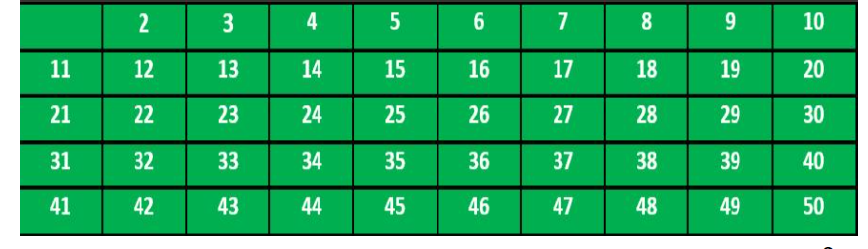
\includegraphics[width=340pt,height=120pt]{slike/sieve-it-0.png}
%\end{figure}

\begin{table}[H]
	\centering
	\begin{tabular}{|c|c|c|c|c|c|c|c|c|c|c} \hline
       & 2 & 3 & 4 & 5 & 6 & 7 & 8 & 9 & 10 \\ \hline
    11 & 12 & 13 & 14 & 15 & 16 & 17 & 18 & 19 & 20 \\ \hline
    21 & 22 & 23 & 24 & 25 & 26 & 27 & 28 & 29 & 30 \\ \hline
    31 & 32 & 33 & 34 & 35 & 36 & 37 & 38 & 39 & 40 \\ \hline
    41 & 42 & 43 & 44 & 45 & 46 & 47 & 48 & 49 & 50 \\ \hline     
	\end{tabular}
    \caption{Inicijalizacija.} \label{eratosten-sieve-it-0}
\end{table}


Dalje, u prvoj iteraciji, nalazimo se na poziciji 2, gdje elemente na pozicijama $2 \cdot k, k=2, \ldots, 50$ eliminišemo kroz sito (kao oni koji nisu prosti, dodijeljujući im vrijednost \emph{False}). Vizuelno, preostali brojevi za ispitivanje su oni neoznačeni:


%\begin{figure}[H]
%	\centering
%	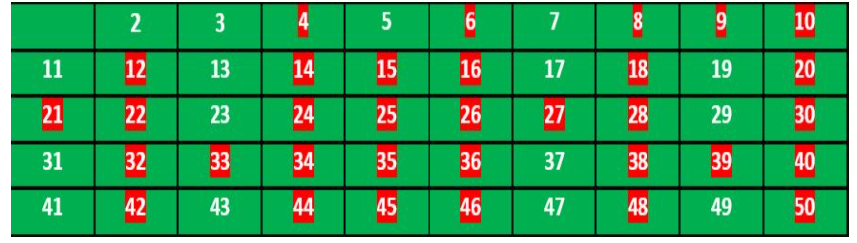
\includegraphics[width=340pt,height=120pt]{slike/sieve-it-1.png}
%\end{figure}

\begin{table}[H]
	\centering
	\begin{tabular}{|c|c|c|c|c|c|c|c|c|c|c} \hline
		& 2 & 3 & \cellcolor{red!30}  4 & 5 & \cellcolor{red!30} 6 & 7 & \cellcolor{red!30} 8 & 9 & \cellcolor{red!30} 10 \\ \hline
		11 &\cellcolor{red!30}  12 & 13 & \cellcolor{red!30} 14 & 15 & \cellcolor{red!30} 16 & 17 & \cellcolor{red!30} \cellcolor{red!30} 18 & 19 & \cellcolor{red!30} \cellcolor{red!30} 20 \\ \hline
		21 & \cellcolor{red!30} 22 & 23 & \cellcolor{red!30} 24 & 25 & \cellcolor{red!30} 26 & 27 &\cellcolor{red!30}  28 & 29 & \cellcolor{red!30} \cellcolor{red!30} 30 \\ \hline
		31 & \cellcolor{red!30} 32 & 33 & \cellcolor{red!30} 34 & 35 & \cellcolor{red!30} 36 & 37 & \cellcolor{red!30} 38 & 39 & \cellcolor{red!30} 40 \\ \hline
		41 & \cellcolor{red!30} 42 & 43 & \cellcolor{red!30} 44 & 45 & \cellcolor{red!30} 46 & 47 &\cellcolor{red!30}  48 & 49 &\cellcolor{red!30}  50 \\ \hline     
	\end{tabular}
        \caption{Eratostenovo sito: iteracija 1.} \label{eratosten-sieve-it-1}
\end{table}



Dalje, u drugoj iteraciji, prelazimo na poziciju 3. Kako je ona označena sa \emph{True} (prost broj), elemente na pozicijama $3\cdot k, k=3, \ldots, 16$ eliminišemo kroz sito (jer nisu prosti). Prelostali brojevi za ispitivanje su oni neoznačeni u narednoj tabeli. 

%\begin{figure}[H]
%	\centering
%	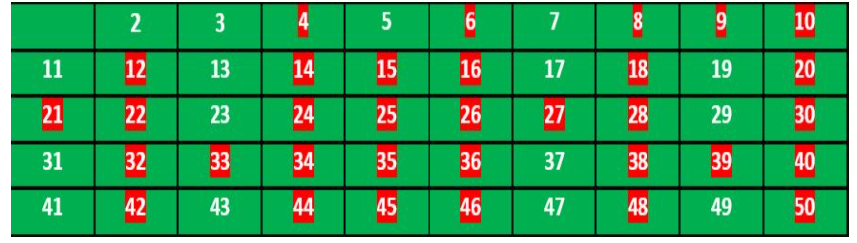
\includegraphics[width=340pt,height=120pt]{slike/sieve-it-1.png}
%\end{figure}

\begin{table}[H]
	\centering
	\begin{tabular}{|c|c|c|c|c|c|c|c|c|c|c} \hline
	& 2 & 3 & \cellcolor{red!30}  4 & 5 & \cellcolor{red!30} 6 & 7 & \cellcolor{red!30} 8 & \cellcolor{red!70} 9 & \cellcolor{red!30} 10 \\ \hline
	11 &\cellcolor{red!30}  12 & 13 & \cellcolor{red!30} 14 & \cellcolor{red!70} 15 & \cellcolor{red!30} 16 & 17 & \cellcolor{red!30} \cellcolor{red!30} 18 & 19 & \cellcolor{red!30} \cellcolor{red!30} 20 \\ \hline
	\cellcolor{red!70} 21 & \cellcolor{red!30} 22 & 23 & \cellcolor{red!30} 24 & 25 & \cellcolor{red!30} 26 & \cellcolor{red!70}  27 &\cellcolor{red!30}  28 & 29 & \cellcolor{red!30} \cellcolor{red!30} 30 \\ \hline
	31 & \cellcolor{red!30} 32 & \cellcolor{red!70} 33 & \cellcolor{red!30} 34 & 35 & \cellcolor{red!30} 36 & 37 & \cellcolor{red!30} 38 &  \cellcolor{red!70}   39 & \cellcolor{red!30} 40 \\ \hline
	41 & \cellcolor{red!30} 42 & 43 & \cellcolor{red!30} 44 & \cellcolor{red!70} 45 & \cellcolor{red!30} 46 & 47 &\cellcolor{red!30}  48 & 49 &\cellcolor{red!30}  50 \\ \hline     
\end{tabular}
        \caption{Eratostenovo sito: iteracija 2.} \label{eratosten-sieve-it-2}
\end{table}

U narednoj iteraciji prelazimo na poziciji 4. Kako to nije prost broj (dakle filtriran prethodno), prelazimo na naredni broj (5), koji je prost, nakon čega ponavljamo operacije opisane prethodnim iteracijama. 


\begin{table}[H]
	\centering
	\begin{tabular}{|c|c|c|c|c|c|c|c|c|c|c} \hline
		& 2 & 3 & \cellcolor{red!30}  4 & 5 & \cellcolor{red!30} 6 & 7 & \cellcolor{red!30} 8 & \cellcolor{red!30} 9 & \cellcolor{red!30} 10 \\ \hline
		11 &\cellcolor{red!30}  12 & 13 & \cellcolor{red!30} 14 & \cellcolor{red!30} 15 & \cellcolor{red!30} 16 & 17 & \cellcolor{red!30} \cellcolor{red!30} 18 & 19 & \cellcolor{red!30} \cellcolor{red!30} 20 \\ \hline
		\cellcolor{red!30} 21 & \cellcolor{red!30} 22 & 23 & \cellcolor{red!30} 24 & \cellcolor{red!90} 25 & \cellcolor{red!30} 26 & \cellcolor{red!30}  27 &\cellcolor{red!30}  28 & 29 & \cellcolor{red!30} \cellcolor{red!30} 30 \\ \hline
		31 & \cellcolor{red!30} 32 & \cellcolor{red!30} 33 & \cellcolor{red!30} 34 & \cellcolor{red!90} 35 & \cellcolor{red!30} 36 & 37 & \cellcolor{red!30} 38 & \cellcolor{red!30} 39 & \cellcolor{red!30} 40 \\ \hline
		41 & \cellcolor{red!30} 42 & 43 & \cellcolor{red!30} 44 & \cellcolor{red!30} 45 & \cellcolor{red!30} 46 & 47 &\cellcolor{red!30}  48 & 49 &\cellcolor{red!30}  50 \\ \hline     
	\end{tabular}
	\caption{Eratostenovo sito: iteracija 3.} \label{eratosten-sieve-it-3}
\end{table}

\section{Faktorizacija broja}

Fundamentalna teorema aritmetike kaže da se svaki prirodan broj $n>1$ može zapisati kao proizvod prostih brojeva na jedinstven način, do na redoslijed faktora. Drugim riječima, za svaki broj $n$ postoje prosti brojevi $p_1,p_2,\ldots,p_k$ i prirodni eksponenti $a_1,a_2,\ldots,a_k$ takvi da vrijedi $n=\prod_{i=1}^{k} p_i^{a_i}.$ Ovaj zapis naziva se \textit{prosta faktorizacija} broja $n$. Na primjer, $
120 = 2^3 \cdot 3 \cdot 5.$

\medskip

Sa algoritamskog stanovišta postavlja se pitanje kako efikasno odrediti prostu faktorizaciju datog broja. Naivan pristup podrazumijeva isprobavanje svih mogućih djelilaca, što za velike brojeve može biti veoma neefikasno.

Efikasniji pristup može se zasnovati na idejama korištenim u Eratostenovom situ. Osnovna ideja je sljedeća: za dati broj $n$ pronađemo njegov najmanji prosti djelilac $p$. Tada vrijedi $
n = p \cdot \frac{n}{p}.$ Nakon toga isti postupak rekurzivno primjenjujemo na broj $n/p$, sve dok ne dođemo do vrijednosti $1$. Na taj način broj postepeno razlažemo na proste faktore.

\medskip

Ovakav pristup prirodno slijedi paradigmu \textit{podijeli pa zavladaj}. Problem faktorizacije broja $n$ svodi se na faktorizaciju manjeg broja $n/p$, pri čemu se rezultat dobija dodavanjem prostog faktora $p$ u konačno rješenje.

\medskip

Da bi se postupak dodatno ubrzao, moguće je unaprijed konstruisati pomoćnu strukturu podataka koja za svaki broj $i$ čuva njegov najmanji prosti faktor. Ova struktura se može izgraditi modifikacijom Eratostenovog sita. Neka je niz $
SPF[0], SPF[1], \ldots, SPF[N]$ (eng. \emph{Smallest Prime Factor}) definisan tako da vrijednost $SPF[i]$ predstavlja najmanji prosti faktor broja $i$. Na primjer, $
SPF[12]=2,
SPF[15]=3,
SPF[49]=7.$ Za proste brojeve vrijedi $ SPF[p]=p. $

Nakon izgradnje niza $SPF$, faktorizacija broja $n$ postaje veoma jednostavna: u svakom koraku uzimamo vrijednost $SPF[n]$, dodajemo je u listu faktora i zamjenjujemo $n$ vrijednošću $
n \leftarrow \frac{n}{SPF[n]}.$

Postupak se ponavlja sve dok ne dobijemo $n=1$.

\medskip

Na primjer, za broj $120$ dobijamo: $
120 \rightarrow 60 \rightarrow 30 \rightarrow 15 \rightarrow 5 \rightarrow 1,$ odnosno proste faktore $2,2,2,3,5,$ što odgovara faktorizaciji $
120 = 2^3 \cdot 3 \cdot 5.$

\medskip

\textit{Kompleksnost algoritma.} Izgradnja niza najmanjih prostih faktora do granice $N$ može se izvršiti u vremenu reda $O(N \log \log N),$  dok se faktorizacija pojedinačnog broja $n$ izvršava u vremenu proporcionalnom broju njegovih prostih faktora, odnosno $O(\log n).$

Zbog toga je ovaj pristup naročito pogodan kada je potrebno faktorisati veliki broj različitih brojeva iz istog intervala.

 Implementacija ovakve (nizovne) strukture je data narednim k\^odom. 
 
 \begin{minted}{python}
 
   def sieve_adaptation(n):
   
       sieve_fact = [0] * (n+1)
       sieve_fact[0] = sieve_fact[1] = 0
       p = 2
       while p <= n:
           if sieve_fact[p] == 0:
       		  index = p * p
       		  while index <= n:
       			 sieve_fact[index] = p
       			 index += p
           p = p + 1
 	
	return sieve_fact
 	
   def factorization(n):
       
       factorize_min_p = sieve_fact(n)
       F = []
       while True: 
           i = factorize_min_p[n]
           if i == 0: 
              F.append(n)
              return F
           else:
              n = n // i
              F.append(i)
       return F  
   
   #ulaz: 
   n = 120
   F = factorization(n)
   print("Lista faktora je: ", F)
 \end{minted} 
 
\textit{Kompleksnost algoritma}. Najskuplja operacija u algoritmu je ada\-ptacija algoritma Eratostenovog sita (funkcija \texttt{sieve\_adaptation}) i ona se izvršava u $O(n \log \log n)$ vremenu. Glavna \texttt{while}-petlja se izvršava u linearnom $O(n)$ vremenu. Dakle, čitav algoritma se izvršava u 
 $O(n \log \log n)$ vremenu.
 
  \section{Izračunavanje binomnih koeficijenata} 
  
  Binomni koeficijenti igraju bitnu ulogu u kombinatorici. Npr. broj različitih grupa od $k$ ljudi može izabrati iz skupa od $n$ ljudi je predstavljen binomnim koeficijentom $\binom{n}{k}$. 
  
  \begin{definition}
  	 Binomni koeficijent $\binom{n}{k}$ gdje je $n, k \in \mathbb{N}, k > 0$  je dat sa 
  	 $$\binom{n}{k} = \frac{n(n-1) \cdots (n-k+1)}{k!}$$
  \end{definition}
  
~ pri čemu je $\binom{n}{0} := 1$. Binomni koeficijent $\binom{n}{1} = n,$ dok je $\binom{n}{n} = 1$ za sve $n \in \mathbb{N}.$ Takođe, ako je $n <k$, vrijedi $\binom{n}{k}=0$.
 
  Lako se može pokazati da vrijedi Paskalova jednakost:
  $$ \binom{n}{k} = \binom{n-1}{k-1} + \binom{n-1}{k},$$
   što nam daje rekurziju za računanje binomnih koeficijenta. Dakle, ako označimo $binom(n, k) = \binom{n}{k}$, vrijedi:
   $$ binom(n, k)= binom(n-1, k-1) + binom(n-1, k).$$
   
   Implementacija rekurzivnog pristupa je data sljedećim k\^odom.
   
   \begin{minted}{python}
     def binom(n, k): 
         if k == 0:
            return 1
         if n < k:
            return 0
         return binom(n-1, k-1) + binom(n-1, k)
   \end{minted}
  \textit{Kompleksnost algoritma}. Faktor grananja rekurzije je 2. To znači da na svakoj narednoj dubini rekurzije imamo (najviše) duplo više rekurzivnih poziva nego je to slučaj na dubini prije.  Kako je dubina rekurzije maksimalno $n$ (vrijednost prvog ili drugog atributa se smanjuje za 1 u narednom pozivu rekurzije), zaključujemo da je maksimalni broj poziva rekurzije eksponenci\-jalan i reda veličine $O(2^n)$. \\
  
  Optimizujmo ovu naivnu implementaciju rekurzije za računanje binomnih koeficijenata.  Jasno se vidi da se većina podproblema rješava više puta u rekurzivnim pozivima. Zbog toga ima smisla upotrebiti princip memoizacije. Označimo strukturu u kojoj čuvamo rješenja matricom $B[i][j]= \binom{i}{j}$. Bazni slučaj je  dat sa $B(n, 0) = 1 = B(n,n)$. Ako je $i < j$, tada je $B[i][j] = 0$. 
  
  Implementacija principa memoizacije za izračunavanje binomnog koefici\-jenta $\binom{n}{k}$ je data narednim k\^odom. 
  
  \begin{minted}{python}
  	
  	def initialization(n, k):
  	    Binom = [[-1] * (k+1)  for _ in range(n+1)] 
  	    return Binom 
  	    
  	def binom_memoization(i, j, Binom): 
  	    
  	    if Binom[i][j] != -1: # već računat
  	       return Binom[i][j] 
  	    if j == 0: 
  	       Binom[i][j] = 1
  	       return Binom[i][j] 
  	    if i < j: 
  	       Binom[i][j] = 0 
  	       return Binom[i][j]
  	       
  	    Binom[i][j] = binom_memoization(i-1, j-1, Binom) 
  	                + binom_memoization(i-1, j, Binom) 
  	    return Binom[i][j]

    #poziv metode:
    n = 10
    k = 4
    Binom = initialization(n, k) 
    n_over_k = binom_memoization(n, k, Binom) 
    print(n_over_k)
    
  \end{minted}  
  
  \textit{Kompleksnost algoritma}.  Kreiranje strukture se izvršava u $O(n\cdot k)$ vremenskoj kompleksnosti. Dalje,  broj podproblema koji se rješavaju je jednak $(n+1) \cdot (k+1)$.  U svakom rekurzivnom pozivu, izvršava se konstantan broj operacija. Sveukupno, kompleksnost algoritma je jednaka $O(n \cdot k)$. 
  
  
  
Katalanovi brojevi pojavljuju se u velikom broju interesantnih kombinatornih problema. U nastavku navodimo nekoliko njihovih poznatih interpretacija.

\begin{itemize}
	\item \textbf{Brojanje putanja na pravougaonoj mreži.} Broj različitih putanja od donjeg lijevog do gornjeg desnog ugla mreže dimenzija $n\times n$, pri čemu se u svakom koraku smije kretati samo udesno ili nagore, a putanja ne smije prelaziti iznad glavne dijagonale (može je samo dodirivati), jednak je $n$-tom Katalanovom broju.
	
	\begin{figure}[H]
		\centering
		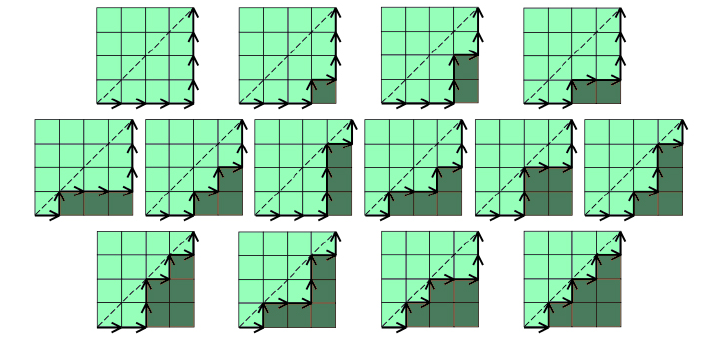
\includegraphics[width=280pt,height=160pt]{slike/catalan-net.png}
		\caption{Putanje na mreži dimenzija $4\times4$.}
		\label{fig:catalan-n-4}
	\end{figure}
	
	\item \textbf{Permutacije bez određenog paterna.} Broj permutacija skupa $\{1,2,\ldots,n\}$ koje ne sadrže patern \texttt{123} (ili, opštije, bilo koji fiksirani patern dužine $3$) takođe je dat Katalanovim brojevima. Na primjer, za $n=3$ dozvoljene su permutacije $	132, 213, 231, 312, 321,$
	dok permutacija \texttt{123} nije dozvoljena. Dakle, postoji ukupno $5$ takvih permutacija, što odgovara vrijednosti $C_3=5$.
	
	\item \textbf{Pravilno ugniježđene zagrade.} Katalanov broj $C_n$ predstavlja broj načina da se formira izraz sa $n$ parova zagrada tako da je svaka otvorena zagrada ispravno zatvorena. Na primjer, za $n=3$ postoji pet takvih izraza:$
	((())), (()()), (())(), ()(()), ()()().$
	
\end{itemize}

Prvih nekoliko Katalanovih brojeva su dati sa nizom: $
1, 1, 2, 5, 14,$ 42, 132, $429, 1430, 4862,\ldots$

Katalanovi brojevi zadovoljavaju sljedeću rekurzivnu relaciju: $
C(0)=1, $ i $
C(n+1)=\sum_{i=0}^{n} C(i),C(n-i),
\qquad n\geq 0.$

Ova rekurzija prirodno proizlazi iz činjenice da se mnogi objekti koji se broje Katalanovim brojevima mogu podijeliti na dva nezavisna dijela, čiji se doprinosi zatim množe i sabiraju preko svih mogućih podjela.

\medskip

Primijenimo sada paradigmu grube sile, odnosno direktnu rekurzivnu implementaciju, za računanje $n$-tog Katalanovog broja. Rekurzija slijedi neposredno iz prethodne formule:

\begin{minted}{python}
	def catalan(n):
	
	    if n == 0:
	        return 1
	        
	    result = 0
	    for i in range(n):
	        result += catalan(i) * catalan(n - 1 - i)
	return result
	
\end{minted}

\textit{Kompleksnost algoritma.} Ovakva implementacija generiše veliki broj ponovljenih izračunavanja istih podproblema. Zbog toga je njena vremenska složenost eksponencijalna. Upravo zbog izraženog preklapanja podproblema, računanje Katalanovih brojeva predstavlja prirodnu primjenu dinamičkog programiranja, koje značajno smanjuje vrijeme izvršavanja memoizacijom ili tabuliranjem prethodno izračunatih vrijednosti.
 Implementacija ovog pristupa je data sljedećim k\^odom. 
 
 \begin{minted}{python}
   def catalan(n):
       if n == 0:
          return 1
       catalan_n = 0 
       for i in range(n): 
           catalan_n += catalan(i) * catalan(n-1-i) 
       return catalan_n
        
 \end{minted}
  
  \emph{Kompleksnost algoritma}. Faktor grananja rekurzije je (najviše) $n$. Dubi\-na rekurzije je $n+1$. Dakle, kompleksnost ovog algoritma je eksponencijalna i iznosi $O(n^n)$. 

Optimizujmo ovaj naivni rekurzivni pristup za računanje Katalanovih brojeva. Kako je primijetno svaki podproblem izražunava iznova više puta, ponovo iskoristimo princip memoizacije. Čuvajmo vrijednost $i$-tog Katalano\-vog broja u nizovnoj strukturi $Cat(i)$.  Svojstvo optimalne podstrukture je dato rekurzijom $Cat(n+1) = \sum_{i=0}^{n} Cat(i) \cdot Cat(n-i).$ Bazni slučaj je dat sa $Cat(0) =1$.

Implementacija memoizacije je data sljedećim k\^odom.

  \begin{minted}{python}
	
	def initialization(n):
	   Cat = [ -1   for _ in range(n+1)  ] 
	   Cat[0]=1
	   return Cat 
	
	def catalan_i(i, Cat): 
	
	    if Cat[i] != -1:
	        return Cat[i]
     
            catalan_i = 0
            for k in range(i): 
                catalan_i += catalan_memoization(k, Cat) *
                     catalan_memoization(i-1-k, Cat)
    
            Cat[i] = catalan_i
            return Cat[i]
    
	#poziv metode:
	n = 10
	Cat = initialization(n) 
	
	cat_n = catalan_n(n, Cat) 
	print(cat_n)
\end{minted}  

\emph{Kompleksnost algoritma}. Dubina rekurzije je (najviše) $n+1$. U svakoj rekurziji, broj iteracija koji se izvršava je linearne kompleksnosti $O(n)$. Prema tome, kompleksnost algoritma je $O(n) \cdot O(n) = O(n^2)$.  \\


 % sretni brojevi, semi-prosti brojevi... 
 
 %Lucky numbers... 
 Posmatrajmo sljedeću proceduru konstruisanja niza brojeva.
 
 \begin{itemize}
 	\item Počinjemo od niza prirodnih brojeva
 	$1, 2, 3, 4, 5, 6, 7, 8$, $9, 10, 11$, $12, 13, 14, 15,$ $16, 17, 18, 19,\ldots 	$
 	
 	\item U prvom koraku brišemo svaki drugi broj. Dobija se niz $1, 3, 5, 7, 9,$ $11, 13, 15, 17, 19,\ldots$
 	
 	\item Iz novodobijenog niza zatim brišemo svaki treći broj, pa dobijamo $
 	1, 3, 7, 9, 13, 15, 19,\ldots
 	$
 	
 	\item Postupak se nastavlja tako što se iz trenutnog niza briše svaki četvrti broj, zatim svaki peti broj itd.
 	
 \end{itemize}
 
 Brojevi koji nikada ne budu obrisani nazivaju se \textit{srećnim brojevima} (eng. \textit{lucky numbers}).
 
 \medskip
 
 U ulazu je dat prirodan broj $n$. Potrebno je utvrditi da li je $n$ srećan broj, odnosno da li će preživjeti prethodno opisani proces eliminacije.
 
 \begin{solution}
 	
 	Posmatrajmo položaj broja $n$ tokom izvođenja postupka. U prvoj iteraciji briše se svaki drugi element niza. Prema tome, svi brojevi djeljivi sa $2$ bivaju uklonjeni.
 	
 	Ako je $n$ paran broj, zaključujemo da će biti obrisan već u prvom koraku i vraćamo rezultat \emph{False}. U suprotnom, broj $n$ preživljava ovu iteraciju. Pošto je uklonjena približno polovina elemenata, njegova nova pozicija postaje
 	
$$
 	n \leftarrow n - \left\lfloor \frac{n}{2} \right\rfloor .
$$
 	
 	U drugoj iteraciji briše se svaki treći element trenutnog niza. Ako je nova pozicija broja $n$ djeljiva sa $3$, broj se uklanja i vraća se rezultat \emph{False}. U suprotnom, broj ostaje u nizu, a njegova pozicija se ažurira na
 	
 	$$
 	n \leftarrow n - \left\lfloor \frac{n}{3} \right\rfloor.
 	$$
 	
 	Opštije, u $i$-toj iteraciji briše se svaki $(i+1)$-vi element trenutnog niza. Neka je trenutna pozicija posmatranog broja jednaka $n$.
 	
 	\begin{itemize}
 		\item Ako je $n < i+1$, broj više ne može biti obrisan ni u jednoj narednoj iteraciji, jer se uklanjaju samo elementi na pozicijama koje su višekratnici broja $i+1$. U tom slučaju vraćamo rezultat \emph{True}.
 		
 		\item Ako je $n$ djeljiv sa $i+1$, broj će biti obrisan u tekućoj iteraciji i vraćamo rezultat \emph{False}.
 		
 		\item U suprotnom, broj preživljava iteraciju, a njegova nova pozicija postaje
 		$$
 		n \leftarrow n - \left\lfloor \frac{n}{i+1} \right\rfloor ,
 		$$
 		jer se prije njega uklanja upravo
 		$\left\lfloor \frac{n}{i+1} \right\rfloor$
 		elemenata.

 		
 	\end{itemize}
 	
 	Postupak se ponavlja sve dok se ne utvrdi da je broj obrisan ili dok njegova trenutna pozicija ne postane manja od koraka eliminacije. U prvom slučaju broj nije srećan, dok u drugom zaključujemo da će preživjeti sve naredne iteracije i da jeste srećan broj.
 	
 \end{solution}
 
 
 Implementacija algoritma je data narednim k\^odom. 
 
 \begin{minted}{python}
 	from math import ceil
 	def lucky_number(n):
 
 	      
 	   for i in range(1, n): #iteracije
 	       if i+1 > ceil(n/i):
 	          return True 
 	       if ceil(n/i)  % (i+1) == 0:
 	          return False
 	   return True       
    
          #poziv funkcije
          print(lucky_number(7)) #True	       
  
 \end{minted}
  
 \end{solution}
 
 \section{Hornerov metod}
 
 \begin{definition}
 	\textbf{\textit{Hornerov metod za izračunavanje vrijednosti polinoma}}. Neka je dat polinom 
 	$P(x)=c_nx^n+c_{n-1}x^{n-1}+\cdots+c_1x+c_0,$ 
 	kao i tačka $x\in\mathbb{R}$. Potrebno je odrediti vrijednost polinoma $P$ u tački $x$. 
 	
 	Pretpostavimo da je polinom predstavljen nizom \texttt{coef}, pri čemu element \texttt{coef[i]} predstavlja koeficijent uz monom $x^{\,n-i}$, za $i\in\{0,\ldots,n\}$.
 	
 \end{definition}
 
 \begin{solution}
 	
 	Posmatrajmo primjer instance: $coef=[1,-3,2,-1], x=3.$ U ovom slučaju riječ je o polinomu $
 	P(x)=x^3-3x^2+2x-1.$ Vrijednost polinoma u tački $x=3$ iznosi $P(3)=27-27+6-1=5.$
 	
 	\medskip
 	
 	Naivan pristup podrazumijeva zasebno računanje svakog stepena $x^i$. Ako se vrijednost $x^i$ računa iterativno, potrebno je $O(i)$ operacija, pa ukupna vremenska složenost evaluacije polinoma iznosi $
 	O(1+2+\cdots+n)=O(n^2).$  	Hornerov metod omogućava izračunavanje vrijednosti polinoma u linearnom vremenu, odnosno u složenosti $O(n)$.
 	
 	Ideju algoritma ilustrujmo na prethodnom primjeru. Polinom možemo zapisati u obliku $P(x)=((x-3)x+2)x-1.$ Drugim riječima, $P(x)=(((c_3x+c_2)x+c_1)x+c_0).$
 	
 	Računanje se odvija sukcesivno:
 	
 	\begin{enumerate}
 		\item Počinje se od vodećeg koeficijenta $c_3=1$.
 		\item Trenutna vrijednost množi se sa $x=3$ i dodaje se naredni koeficijent: $1\cdot 3+(-3)=0.$
 		\item Dobijena vrijednost ponovo se množi sa $x$ i dodaje se sljedeći koeficijent: $ 0\cdot 3+2=2.$
 		\item Postupak se ponavlja: $2 \cdot 3+(-1)=5.$
 	\end{enumerate}
 	
 	Dobijamo konačnu vrijednost polinoma $	P(3)=5.$
 	
 	\medskip
 	
 	U opštem slučaju vrijedi identitet $$
 	c_nx^n+c_{n-1}x^{n-1}+\cdots+c_1x+c_0
 	=(\cdots((c_nx+c_{n-1})x+c_{n-2})x+\cdots+c_1)x+c_0.
 	$$
 	
 	Na ovaj način izbjegava se eksplicitno računanje stepena broja $x$, pa se polinom evaluira korištenjem samo $n$ množenja i $n$ sabiranja.
 	
 	\medskip
 	
 	\textit{Bazni slučaj}. Ako je $n=0$, polinom se svodi na konstantu $	P(x)=c_0,$ 	pa algoritam neposredno vraća vrijednost $c_0$.
 	
 	\medskip
 	
 	\textit{Kompleksnost algoritma}. Hornerov metod izvršava tačno $n$ množenja i $n$ sabiranja, pa je njegova vremenska složenost jednaka $
 	O(n),$	dok je prostorna složenost $O(1)$.
 \end{solution}
 
 Implementacija Hornerovog metoda je data narednim k\^odom. 
	 
	 \begin{minted}{python}
	 	 def horner_metod(coef, x):
	 	   
	 	     rezultat = 0
	 	     for c in coef:
	 	         rezultat = rezultat * x + c
	 	     
	 	     return rezultat
	 	 
	 	 # poziv funkcije
	 	 # Evaluacija:  x^3 - 3 x^2 + 2 x -1, x = 3
	 	 coef = [1, -3, 2, -1]
	 	 x = 3
	 	 print(horner_metod(coef, x))
	 \end{minted}

\textit{Kompleksnost algoritma.}  Jasno je da je najintenzivniji dio izvršavanja operacija smješten u \texttt{for}-petlju. Svaka iteracija se izvršava u konstantnom vremenu, pa zaključujemo da se algoritam izvršava u linearnom vremenu, tj. $O(n)$.  
\end{solution}
 
 %https://www.geeksforgeeks.org/sieve-of-atkin/ ==> SIEVE OF ATKIN ==> ako bude trebalo dodati...
 
 \section*{Zadaci}
 
 \begin{enumerate}
 	\item Broj je poluprost (eng. \textit{semiprime}) ako se može predstaviti
 	kao proizvod dva (ne obavezno različita) prosta broja. Npr. $4, 6, 9, 10, \ldots$ su neki od poluprostih brojeva. Konstruisati (efikasan) algoritam koji ispituje da li je broj poluprost.
 	\item Broj je savršen akko je jednak zbiru svojih djelilaca (ne računajući njega samog). Npr. 6 i 28 su savršeni jer je $6 = 1 + 2 + 3; 28 = 1 + 2 + 4 + 7 + 14$. Napisati program koji ispituje da li je broj savršen korištenjem Eratostenovog sita. Kolika je vremenska složenost algoritma? Uporediti ovaj algoritam sa algoritamskom paradigmom brutalne sile.
 	\item Broj je ružan akko su mu jedini prosti faktori 2 ili 3 ili 5. Niz prvih ružnih brojeva je dat sa $1, 2, 3, 4, 5, 6, 8, 9, 10, 12, 15, \ldots$ (1 je po
 	konvenciji uključen). U ulazu je  dat broj $n$. Izračunati $n$-ti ružni broj. Koristiti paradigmu dinamičkog programiranja.
 	\item Sfenički brojevi su pozitivni cijeli brojevi koji se dobijaju kao proizvod tačno 3 različita prosta faktora. Npr. $30, 42, 66, 70, 78,$ $102, 105, 110, 114, \ldots$ su neki od takvih brojeva. U ulazu je dat broj $n$. Ispitati da li je on sfenički? 
 	
 	\textit{Primjer}. $30=2 \cdot 3 \cdot 5$ jeste sfenički, dok $60 = 2^2 \cdot 3 \cdot 5 $ nije sfenički. 
 	\item Za broj se kaže da je slobodan od kvadrata ako ga nijedan
 	prosti faktor ne dijeli više od jednom, tj. najveći stepen prostog
 	faktora koji dijeli $n$  je jedan.  Prvih nekoliko slobodnih kvadrata brojeva su $$1, 2, 3, 5, 6, 7,
 	10, 11, 13, 14, 15, 17, 19, 21.$$   Na ulazu je dat broj $n$. Ispitati da li je on broj 	slobodnog kvadrata.
 	\item Neka je dat broj $n$. Ispitati da li je to \textit{lažni} broj ili ne.
 	Pod lažnim brojem podrazumijevamo složeni broj, čiji je zbir cifara jednak zbiru cifara njegovih različitih prostih faktora.%https://www.geeksforgeeks.org/hoax-number/
 	
 	\item Dat je skup od $n$ elemenata, pronaći broj načina particionisanja broja (Belovi brojevi). Implementirati efikasnu proceduru računanja ovakvih brojeva u zavisnosti od $n$.  %https://www.geeksforgeeks.org/bell-numbers-number-of-ways-to-partition-a-set/
 \end{enumerate}